% discuss survey comments... already seen -- similar but not exact

In this section we discuss the algorithms evaluated in our two online
trials\footnote{All code used in these experiments is available at
\url{http://code.google.com/p/social-recommendation/}.  The conditions
of our ethics approval \#2011/142 from the Australian National
University for conducting human trials on Facebook require our
privacy policy
(\url{http://dmm.anu.edu.au/linkr/website/pp.php}) to
prohibit public sharing of data collected during these experiments.}
and additional analysis regarding trends and patterns in our social
recommendation setting.

\subsection{First Trial}

In our first trial, our objective was to evaluate four CF and SCF
approaches to establish which was the most promising direction for
SCF extension:
\begin{enumerate}
\item {\bf $k$-Nearest Neighbor (KNN)}: Section~\ref{sec:nn} $(N\sql=\sql50)$.
\item {\bf Support Vector Mach. \sq(SVM)}: Section~\ref{sec:cbf} $(C\sql=\sql2)$.
\item {\bf Matchbox (Mbox)}: simple Matchbox CF %Optimization of the $L_2$ regularized Matchbox objective:
$$\Obj_\pmcf + \lambda \Obj_\ru + \lambda \Obj_\rv \, (\lambda\sql=\sql10^2)$$
\item {\bf Social Matchbox (Soc. Mbox)}: %Optimization of the 
%$L_2$ and 
feature-based \emph{socially regularized} Matchbox SCF
$$\Obj_\pmcf + \lambda_\rs \Obj_\rs + \lambda \Obj_\ru + \lambda \Obj_\rv \, (\lambda_\rs\sql=\sql10^{-3}, \lambda\sql=\sql10^2)$$
\end{enumerate}
KNN and MBox may be viewed as pure CF methods.  As discussed previously,
both SVM and Soc. Mbox may be viewed as SCF methods; all objectives
for these were given in Section~\ref{sec:NewObjFuns}
and were both optimized via gradient descent as outlined
in Appendix~\ref{app:Derivatives}.  

The first live user trial was run from August 25, 2011 to October 13, 2011 
with 108 users and yielded 2,493 combined like and 
dislike ratings of recommended
links over the 49 day period.  Algorithms were assigned randomly to the
users with assignment counts shown in Table~\ref{tab:Assigned1} (left).

%%%%%%%%%%%%%%%%%%%%%%%%%%%%%%%%%%%%%%%%%%%%%%%%%%%%%%%%%%
\begin{table}[t!]
\centering \footnotesize
\begin{tabular}{|l|l|l|l|l|l|}
\multicolumn{6}{c}{\bf Trial 1 -- Aug. 25, 2011 to Oct. 13, 2011 } \\ \hline
 & {\rm SMB} & {\rm MB} & {\rm SVM} & {\rm KNN} & {\rm Total}\\ \hline
{\rm Users All} & 26 & 26 & 28 & 28 & 108 \\
{\rm Users $\geq 10$} & 13 & 9 & 13 & 4 & 39 \\
{\rm Users $\geq 30$} &  9 & 3 & 11 & 2 & 25 \\ \hline
{\rm Ratings All}  & 819 & 526 & 901 & 242 & 2508 \\
{\rm Ratings $\geq 10$} & 811 & 505 & 896 & 228 & 2440 \\
{\rm Ratings $\geq 30$} & 737 & 389 & 851 & 182 & 2159 \\ \hline %23 \% have 86\% ratings
{\rm Clicks All}   & 383 & 245 & 413 & 218 & 1259 \\ \hline
\multicolumn{6}{c}{} \\ 
\multicolumn{6}{c}{\bf Trial 2 -- Oct. 14, 2011 to Feb. 10, 2012} \\ \hline
 & {\rm SMB} & {\rm Sp.MB} & {\rm Sp.CP} & {\rm SHyb.} & {\rm Total}\\ \hline
{\rm Users All} & 27 & 27 & 29 & 28 & 111 \\
{\rm Users $\geq 10$} & 15 & 11 & 8 & 12 & 46 \\
{\rm Users $\geq 30$} & 12 & 9  & 5 & 10 & 36 \\ \hline
{\rm Ratings All}  & 1434 & 882 & 879 & 614 & 3809 \\ 
{\rm Ratings $\geq 10$} & 1411 & 878 & 863 & 602 & 3754 \\
{\rm Ratings $\geq 30$} & 1348 & 850 & 802 & 570 & 3570 \\ \hline %23 \% have 86\% ratings
{\rm Clicks All}   & 553  & 320 & 278 & 199 & 1350 \\ \hline
\end{tabular}
\caption{\footnotesize
Number of users assigned per algorithm in the first and
second trials.  $\geq 10$ ($\geq 30$) indicates data for
the subset of users with at least 10 (30) ratings.}
\label{tab:Assigned1}
\end{table}
%%%%%%%%%%%%%%%%%%%%%%%%%%%%%%%%%%%%%%%%%%%%%%%%%%%%%%%%%%

As shown in Figure~\ref{fig:OnlineResult1}, Soc. Mbox was the
best performing algorithm in the first trial and in fact was the only
algorithm to receive more like ratings than dislike ratings. 
This suggests that using social regularization in conjunction with
MF-based CF does indeed provide more useful information than simple
MBox without social regularization.  We also note a
significant drop in performance between recommending friend links and
recommending non-friend links, indicating that users had a bias to
like links recommended by friends more (importantly, we note that
users could see the names and comments of friends whose links were recommended).
%%%%%%%%%%%%%%%%%%%%%%%%%%%%%%%%%%%%%%%%%%%%%%%%%%%%%%%%%%
\begin{figure*}[t!]
\centering
\subfigure{\includegraphics[scale=0.28]{img_new/live-likes1-orig.eps}}
\subfigure{\includegraphics[scale=0.28]{img_new/live-friend-likes1-orig.eps}}
\subfigure{\includegraphics[scale=0.28]{img_new/live-nonfriend-likes1-orig.eps}}
\caption{Stacked bar graphs of online results for the first 
user trial.  The fraction of likes is displayed above 
the fraction of dislikes.  (left) all links, (center) friend links,
(right) non-friend links.  The 95\% confidence interval on all 
results is $< \pm 0.02$ so all differences are signficant
except for MBox and SVM in the center and the virtual tie
between three algorithms on the right.}
\label{fig:OnlineResult1}
\end{figure*}
%%%%%%%%%%%%%%%%%%%%%%%%%%%%%%%%%%%%%%%%%%%%%%%%%%%%%%%%%%

%%%%%%%%%%%%%%%%%%%%%%%%%%%%%%%%%%%%%%%%%%%%%%%%%%%%%%%%%%
%%%%%%%%%%%%%%%%%%%%%%%%%%%%%%%%%%%%%%%%%%%%%%%%%%%%%%%%%%

\subsection{Second Trial} 

For the second online trial, we again chose four algorithms to
randomly assign to the LinkR application users.  Social Matchbox
was included again as a baseline since it was the best performing
algorithm in the first trial.  The remaining three algorithms
were all relatively orthogonal extensions (or variants) of Social Matchbox
based on the \emph{three novel objective functions} defined in 
Section~\ref{sec:newobjfun_defs}:
\begin{itemize}
\item {\bf Social Matchbox (Soc. Mbox)} : unchanged.
\item {\bf Spectral Matchbox (Spec. Mbox)}: 
$$\Obj_\pmcf + \lambda_\rss \Obj_\rss + \lambda_\ru \Obj_\ru + \lambda_\rv \Obj_\rv$$
%Matchbox MF + Social Spectral Regularization + L2 $U$ Regularization + L2 $V$ Regularization
\item {\bf Social Hybrid (Soc. Hybrid)}: 
$$\Obj_\phy + \lambda_\rs \Obj_\rs + \lambda_\ru \Obj_\ru + \lambda_\rv \Obj_\rv + \lambda_rw \Obj_\rw$$
%Hybrid + Social Regularization + L2 $U$ Regularization + L2 $V$ Regularization + L2 $\w$ Regularization
\item {\bf Spectral Co-preference (Spec. CP)}: 
$$\Obj_\pmcf + \lambda_\rscs \Obj_\rscs + \lambda_\ru \Obj_\ru + \lambda_\rv \Obj_\rv$$
%Matchbox MF + Social Co-preference Spectral Regularization + L2 $U$ Regularization + L2 $V$ Regularization
\end{itemize}
All objectives are defined in Section~\ref{sec:NewObjFuns} 
and optimized via gradient descent as outlined
in Appendix~\ref{app:Derivatives}.  

The second trial with the above algorithms ran from Oct. 14, 2011 to
Feb. 10, 2011 as shown in Table~\ref{tab:Assigned1} (bottom); on the
start of the second trial, users were notified that they would be
randomly assigned to new algorithms and encouraged to re-engage with
the LinkR App if they had not been using it.

%%%%%%%%%%%%%%%%%%%%%%%%%%%%%%%%%%%%%%%%%%%%%%%%%%%%%%%%%%%%%%%%%%%%%%%%%
\begin{figure*}[t!]
\centering
\subfigure{\includegraphics[scale=0.28]{img_new/live-likes2-Feb10.eps}}
\subfigure{\includegraphics[scale=0.28]{img_new/live-friend-likes2-Feb10.eps}}
\subfigure{\includegraphics[scale=0.28]{img_new/live-nonfriend-likes2-Feb10.eps}}
\caption{Stacked bar graphs of online results for the second
user trial.  The fraction of likes is displayed above 
the fraction of dislikes.  (left) all links, (center) friend links,
(right) non-friend links. The 95\% confidence interval on all 
results is $< \pm 0.026$ so all differences except Spec. Mbox
and Soc. Hybrid in the center graph are significant. }
\label{fig:online2}
\end{figure*}
%%%%%%%%%%%%%%%%%%%%%%%%%%%%%%%%%%%%%%%%%%%%%%%%%%%%%%%%%%%%%%%%%%%%%%%%%

Results for the second trial are 
shown in Figure~\ref{fig:online2}, following are the key observations:
\begin{itemize}
\item Soc. MBox did not perform as well in the second trial as it had
in the first trial.  We left Soc. MBox unchanged between the first and
second trials so that it could be used as a fixed comparative
baseline.  However, we hypothesize that Soc. MBox may have performed
better (comparably to its first trial performance) if $\lambda_rs$ and
$\lambda$ were better tuned for the amount of data in the second
trial.  In the following table, we show the accuracy of Soc. MBox at
predicting link likes/dislikes on second trial data, training on 75\%
of the data and testing on the remaining 25\%:\\
$\qquad$\\
\begin{tabular}{| l | l | l | l | l | l |} \hline
%& \multicolumn{5}{|c|}{$\lambda_\rs$} \\ \hline
& {\rm $\lambda_\rs \sql = \sql 10^{-1}$}  \sqm\sqm & {\rm $\sql=\sql10^{-2}$}  \sqm\sqm & {\rm $\sql=\sql10^{-3}$} \sqm\sqm & {\rm $\sql=\sql10^{-4}$} \sqm\sqm & {\rm $\sql=\sql10^{-5}$} \sqm \\ \hline
\sq {\rm $\lambda$=$10^1$} \sqm\sq & 0.325 & 0.307 & 0.301 & 0.437 & 0.540 \\
\sq {\rm $\lambda$=$10^2$} \sqm\sq & 0.306 & 0.301 & {\bf 0.300} & 0.295 & 0.300 \\
\sq {\rm $\lambda$=$10^3$} \sqm\sq & 0.297 & 0.301 & 0.307 & 0.300 & 0.301 \\
%\sqm {\rm $\lambda$=$10^4$} \sqm & 0.301 & 0.301 & 0.301 & 0.339 & 0.363 \\
 \hline
\end{tabular}
Here we show the parameters used in the second trial in bold which
achieves a prediction accuracy of 0.300, but with both $\lambda$ and
$\lambda_\rs$ reduced, we note a substantial improvement to 0.436 and
0.540.  Intuitively, less regularization is needed in the presence of
the additional data in the second trial and the drastic performance
differential here reinforces the importance of careful (and frequent)
parameter re-tuning for optimal recommendation performance.

\item Spec. Mbox clearly performed the best in the second trial 
and this suggests that spectral social regularization is likely a
better method of regularization than the original social
regularization variant.  Taking into account possible suboptimal
performance of Soc. Mbox in the second trial, we note that even when
(i) extrapolating from the previous parameter tuning results to
conjecture that Soc. Mbox may have achieved up to 54\% accuracy at
predicting overall likes or (ii) alternately conjecturing a similar
performance of 50\% for Soc. Mbox as in the first trial, both
speculative results would still indicate significantly lower accuracy
of overall likes prediction for Soc. Mbox in the second trial compared to
Spec. MBox's impressive 66\%.

\item Soc. Hybrid statistically ties Spec. MBox at 
recommending friend links (where it can learn user-to-user information
diffusion), but performs less well on non-friend links (where there is
no such diffusion).
%However, given the modeling complexity of
%Soc. Hybrid, which in our evaluation requires training tens of
%thousands of weights $\vec{w}$ for $\f_{\x,\y}$ as outlined in
%Section~\ref{sec:fxy_def}, 
Interestingly, these results suggest that the space- and
compution-efficient low-dimensional latent user feature learning of
Spec. MBox can recommend friend links just as well Soc. Hybrid's 
modeling of explicit user-to-user information diffusion, which is
important to note given the substantial computational and space
overhead of the latter.

\item Spec. CP did not perform as well as most other algorithms
across the different evaluation metrics.  Compared to the simpler
regularization by social interaction used in the other algorithms,
we might conjecture that the relative abundance of interaction data
provides a more reliable social regularizer than the somewhat sparse
copreference data.
\end{itemize}

%%%%%%%%%%%%%%%%%%%%%%%%%%%%%%%%%%%%%%%%%%%%%%%%%%%%%%%%%%
%%%%%%%%%%%%%%%%%%%%%%%%%%%%%%%%%%%%%%%%%%%%%%%%%%%%%%%%%%

\subsection{User Behavior Analysis}

\label{sec:behavior}

Here we briefly analyze user behavior during both trials of the Facebook
LinkR App that can be helpful in building future SCF systems.

\subsubsection{Click evidence}

In Figure~\ref{fig:click_evidence}(a), we observe the ratings of links
that users clicked on.  The most important thing we notice 
here is that even though users
clicked on a link, they were somewhat likely to rate it as a dislike.

One might hypothesize that perhaps users clicked on links more often
with no description to find out what they were and most often disliked
them --- this might explain the high number of dislikes for clicked
links.  However, examining both Figures~\ref{fig:click_evidence}(b)
and (c), we observe that whether a description was present had a
relatively minor impact on whether a link was clicked or liked, so we
cannot infer that all the disliked links were simply the ones lacking
a description.

Then the insight from this analysis is extremely important 
for SCF recommendation design because it states that click data is a somewhat 
weak indicator of likes (roughly $\frac{1}{3}$ of clicks are disliked)
and thus explicit feedback should be used if at all possible.

%%%%%%%%%%%%%%%%%%%%%%%%%%%%%%%%%%%%%%%%%%%%%%%%%%%%%%%%%%
\begin{figure*}[t!]
\centering
\subfigure[]{\includegraphics[scale=0.31]{img_new/clicked-likes.eps}}
\hspace{-4.2mm}
\subfigure[]{\includegraphics[scale=0.31]{img_new/description-clicked.eps}}
\hspace{-4.2mm}
\subfigure[]{\includegraphics[scale=0.31]{img_new/description-liked.eps}}
\hspace{-4.2mm}
\subfigure[]{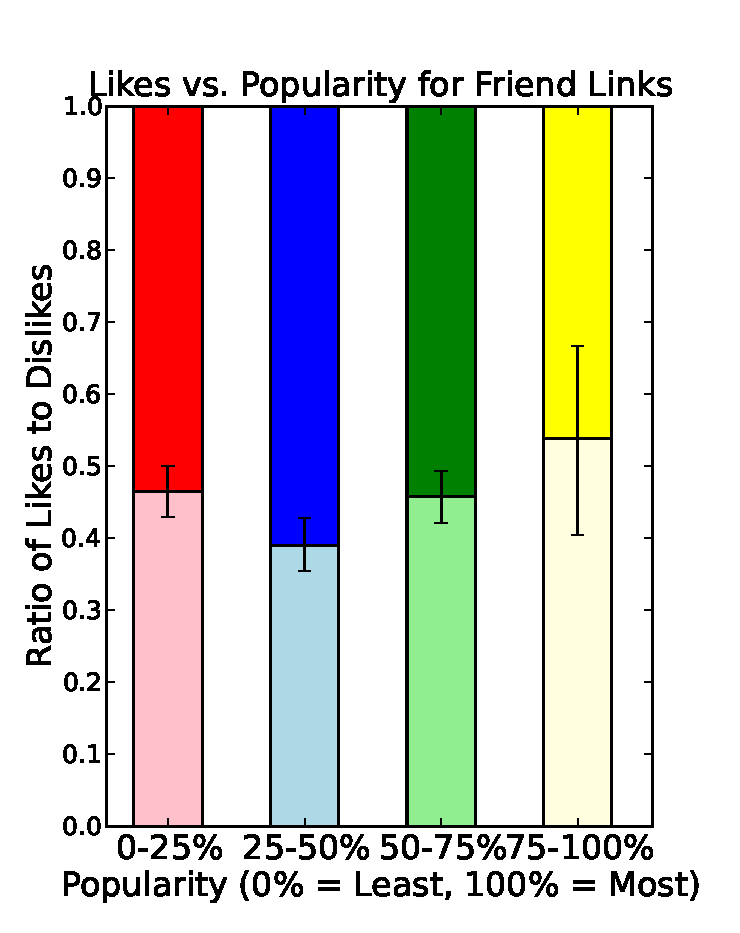
\includegraphics[scale=0.31]{img_new/friend-popularity.eps}}
\hspace{-3.3mm}
\subfigure[]{\includegraphics[scale=0.31]{img_new/non-friend-popularity.eps}}
%\vspace{-3mm}
\caption{Stacked bar graphs of online results for the first 
user trial.  The fraction of likes (or clicks) is displayed above 
the fraction of dislikes (or non-clicks) -- and above the fraction of not-rated
links for the left-most figure.  
(left) ratings for clicked links, (center) click rates if
text description not present, 
(right) percentage liked if click description not present.
Stacked bar graphs of online results for the first 
user trial.  The fraction of likes is displayed above the fraction of
dislikes.  Shown are the ratings vs. quartile of popularity for (left)
friend and (right) non-friend links.
Stacked bar graphs of online results for the first 
user trial.  The fraction of likes is displayed above the fraction of
dislikes.  Shown are the ratings vs. quartile of popularity for (left)
friend and (right) non-friend links.
}
\label{fig:click_evidence}
\end{figure*}
%%%%%%%%%%%%%%%%%%%%%%%%%%%%%%%%%%%%%%%%%%%%%%%%%%%%%%%%%%

\subsubsection{Impact of Popularity}

In Figure~\ref{fig:click_evidence}(d,e) we analyze the impact of global link
popularity (in terms of total shares on Facebook) 
on how much Facebook LinkR App users liked a link.
The trend is clear for both friend (left) and non-friend (right)
links: users tend to like the most popular (top quartile) 
links the least, or at least as much as the least popular (bottom quartile)
links.  In general users tended to prefer links that were somewhat
popular (second highest quartile).  From this we can infer that
link popularity should not be used too heavily in determining link
recommendations since clearly the most popular links are not liked
the most on average.

%%%%%%%%%%%%%%%%%%%%%%%%%%%%%%%%%%%%%%%%%%%%%%%%%%%%%%%%%%
%\begin{table}[t!]
%\centering
%\footnotesize
%\caption{There were two parameters tuned.  The main objective
%was fixed at 1 since it is only the relative ratios of parameters
%that matter.  Here we see that for low $\lambda$ and $\beta$ we
%get better performance, as would be expected since there is now
%more data and we can let the main objective have a greater
%influence on the result.}
%\label{fig:tuning}
%\end{table}
%%%%%%%%%%%%%%%%%%%%%%%%%%%%%%%%%%%%%%%%%%%%%%%%%%%%%%%%%%


%%%%%%%%%%%%%%%%%%%%%%%%%%%%%%%%%%%%%%%%%%%%%%%%%%%%%%%%%%
\begin{table}[t!]
\centering
\footnotesize
\begin{tabular}{c c}
\hspace{-3mm} 
\begin{tabular}{|l|r|r|} 
\multicolumn{3}{c}{Individual Link Comments} \\ \hline
Comment Type & \# & \% \\ \hline % 241 total
not interested & 88 & 36.5\% \\
wrong language & 37 & 15.4\% \\
really liked it! & 35 & 14.5\% \\
bad YouTube & 25 & 10.4\% \\
seen it	already & 25 & 10.4\% \\
problem / dead & 20 & 8.3\% \\
not current & 7 & 2.9\% \\	
miscellaneous & 4 & 1.7\% \\
%problem	& 4 & \% \\
%dead & 16 & \% \\
\hline
\end{tabular}
&
\hspace{-3mm} \begin{tabular}{|p{3.34cm}|}
\multicolumn{1}{p{3.34cm}}{User Survey Comments}\\ \hline
want more control over recommendations made (music, blogs, news)\\ \hline
%and specific preferences (heavy metal vs. rap music)\\ \hline
want option to see $> 3$ recommendations \\ \hline
links need description / context or explanation of recommendation \\ \hline 
more variety, diversity\\ \hline
\end{tabular}
\end{tabular}
\caption{Individual link comments (aggregated) and 
and overall user survey comments (paraphrased).}
\label{table:survey}
\end{table}
%%%%%%%%%%%%%%%%%%%%%%%%%%%%%%%%%%%%%%%%%%%%%%%%%%%%%%%%%%
